%!TEX root = ../Lab-report.tex

\section{Рябь}
Рябь возникает из-за усечения сигнала во временной области. Устранить этот эффект нельзя, но можно минимизировать, увеличивая временную область $[a, b] $ или частоту дискретизации сигнала. \\
\begin{figure}[h]
\centering
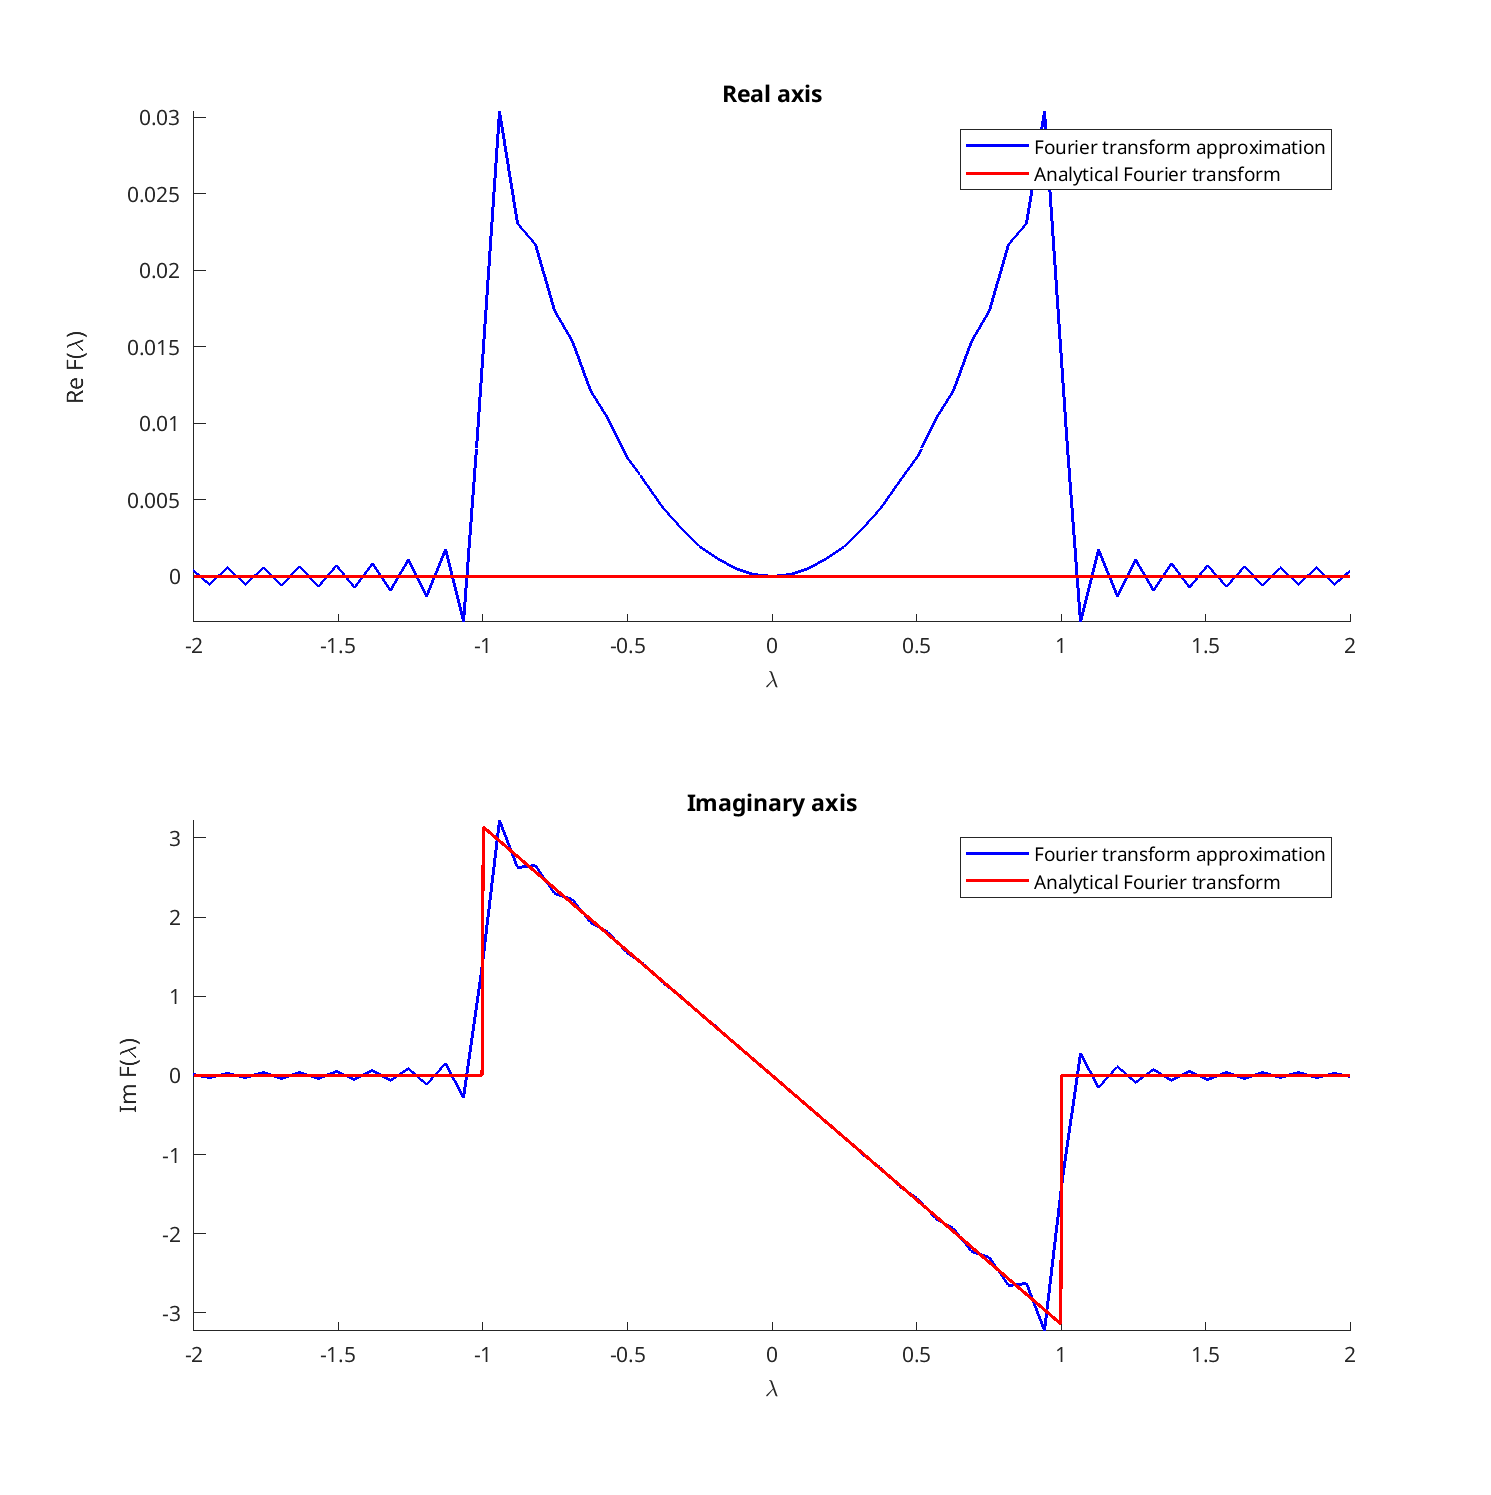
\includegraphics[width=\textwidth, height=0.7\textheight]{Gibbs}
\caption{$ T = 100, \Delta t = 0.05, t \in [-50; 50] $}
\end{figure}

\begin{figure}[h]
\centering
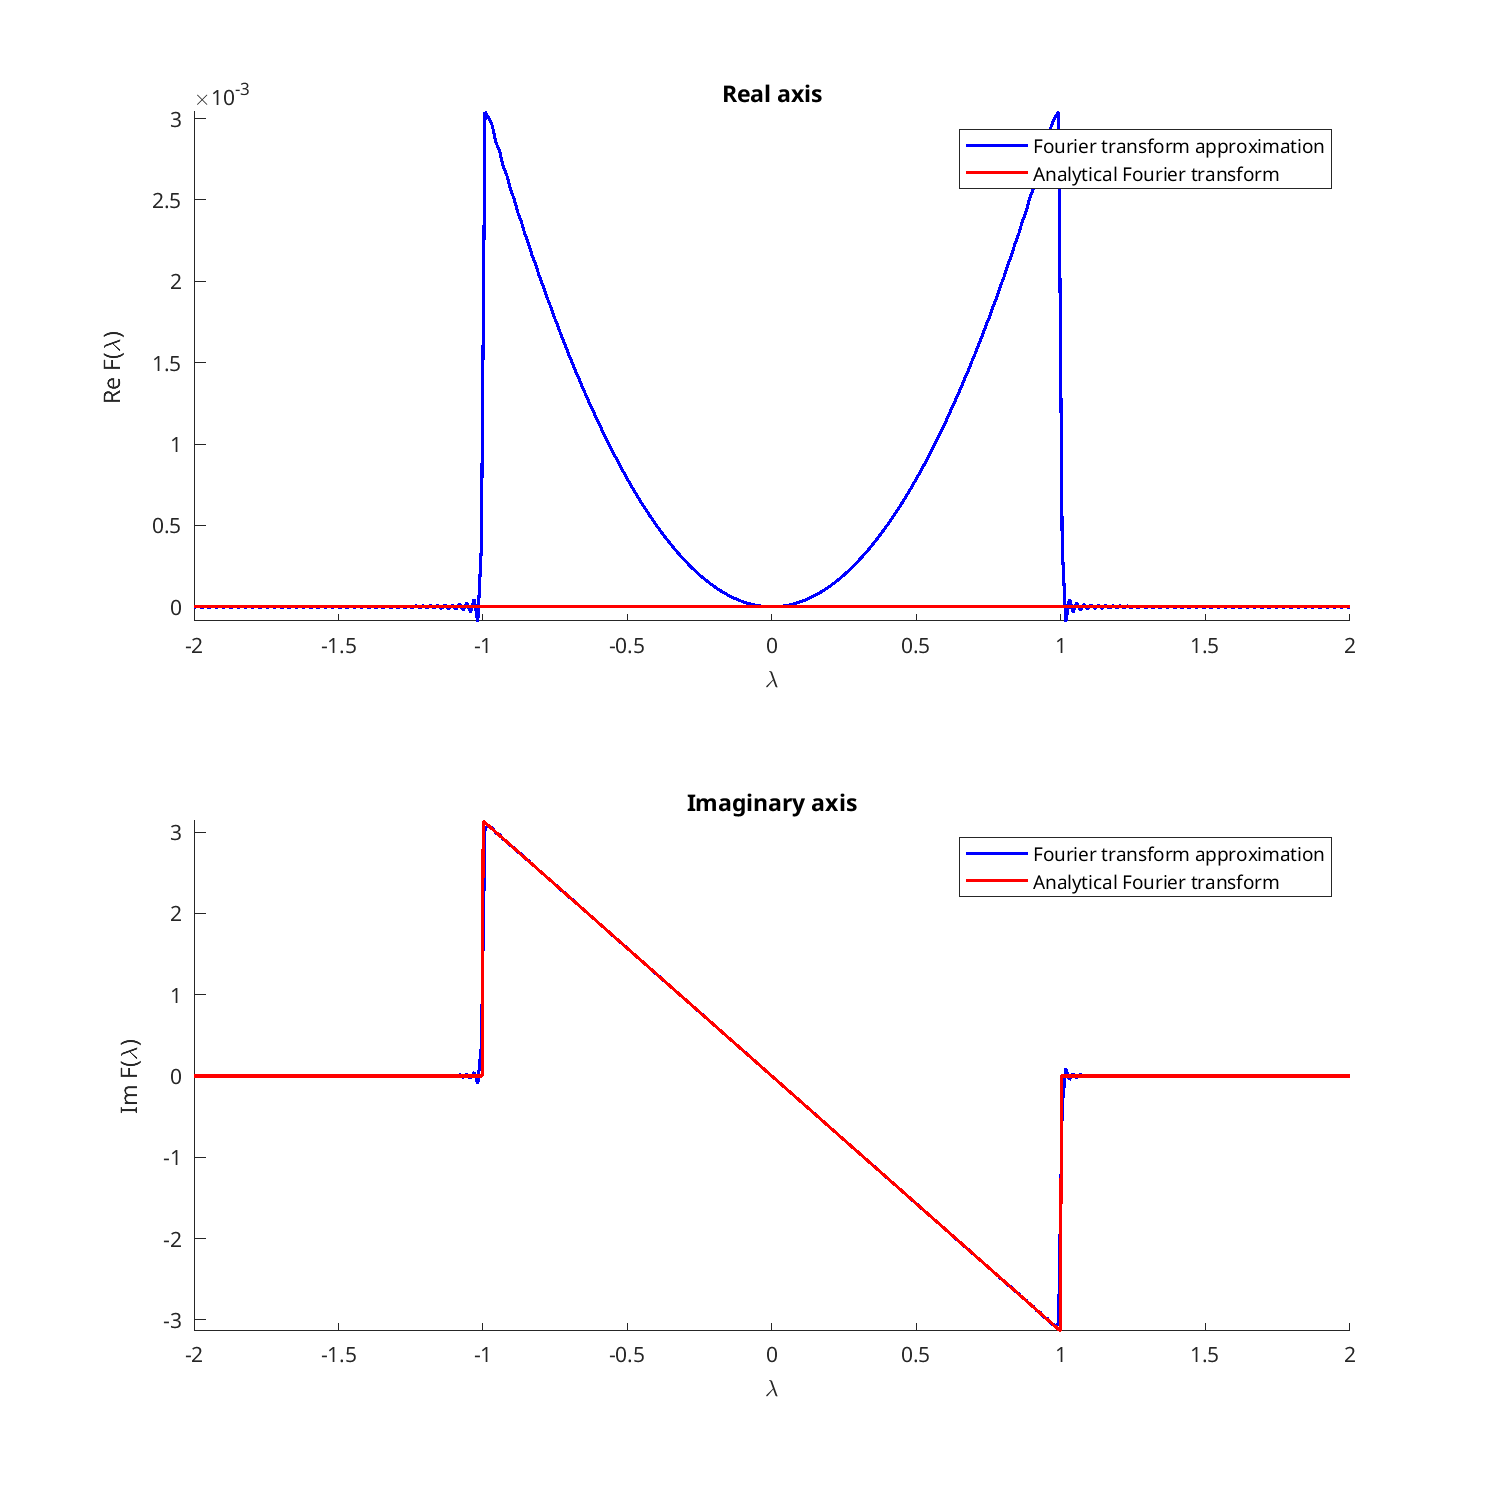
\includegraphics[width=\textwidth, height=0.7\textheight]{Gibbs-2}
\caption{$ T = 500, \Delta t = 10^{-3}, t \in [-250; 250] $}
\end{figure}